\documentclass[a4paper,11pt]{article}
\usepackage[utf8]{inputenc} 
\usepackage[spanish]{babel} 
\usepackage{hyperref}
\usepackage{amsmath}
\usepackage{mathtools}
\everymath{\displaystyle}
\usepackage{graphicx}

\begin{document}
\title{Mi nuevo artículo} 
\author{Rodrigo Díaz Alfaraz}
\date{21 octubre 2018}
\maketitle

\paragraph*{Mi nuevo artículo}

\paragraph*{Autor}
Rodrigo Díaz Alfaraz

\section*{Resumen} 
Enlace al repositorio:
\url{https://github.com/rdalfaraz/proyecto_final} Es la url del repositorio donde se va a alojar este proyecto.
\paragraph*{Palabras clave}

GIT, LATEX, GITHUB, JABREF

\section*{Introducción}
Este articulo trata de recopilar los conocimientos adquiridos en el curso. 

\section*{Estado del arte}
\cite{Espanola2015a}
En el ámbito de la investigación científica, el estado del arte de un artículo hace referencia al estado último de la materia en términos de I+D, refiriéndose incluso al límite de conocimiento humano público sobre la materia.

\section*{Imágenes y tablas}
En este curso se han estudiado los siguientes módulos:

\begin{table}
\centering
\begin{tabular}{|c|c|}
\hline
Módulo 1 & Git básico \\
\hline
Módulo 2 & Git Avanzado. Solución de problemas y aspectos avanzados \\
\hline
Módulo 3 & LaTeX básico \\
\hline
Módulo 4 & LaTeX. Avanzando en contenido y forma \\
\hline
Módulo 5 & Aspectos avanzados de LaTEX \\
\hline
\end{tabular}
\end{table}



\begin{figure} 
\centering

\includegraphics[width=25mm]{git.png}
\section{Imagen de Git}
\end{figure}


\begin{figure} 
\centering
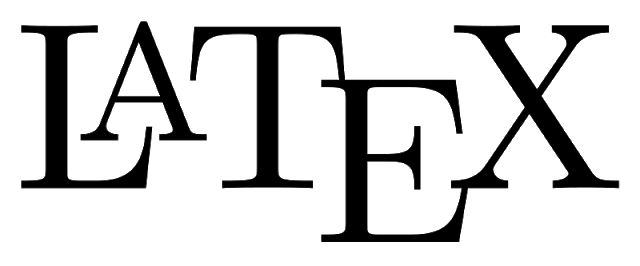
\includegraphics[width=25mm]{LaTeX_logo.png}
\section{Imagen de Latex}
\end{figure}

\section*{Fórmulas}
\paragraph{En esta sección se van a mostrar una serie de fórmulas:}
$$\cos (2\theta)= \cos^2 \theta - \sin^2 \theta$$

$$\lim\limits_{x \to \infty} \exp(-x) = 0$$

\section*{Bibliografía}


\bibliography{referencias}
\bibliographystyle{plain}
\nocite{*}

\end{document}
